\begin{exercício}{Placas paralelas parcialmente preenchidas com material dielétrico}{exercício4}
    Considere duas placas metálicas quadradas de lado \(L\) e espessuras desprezíveis. As placas estão paralelas e separadas por uma distância \(d\). Assuma que os planos das placas são paralelos ao plano \(xy\), que a placa inferior (superior) está em \(z = 0\) (\(z = d\)) e que estão orientadas como mostra a figura abaixo.

    \begin{center}
        \begin{tikzpicture}[scale=0.8, every node/.style={scale=0.8}]
            \draw[-stealth] (-3.,0,0) -- (3.,0,0) node[below] {$y$};
            \draw[-stealth] (0,-.5,0) -- (0,2.5,0) node[left] {$z$};
            \draw[-stealth] (0,0,-2.5) -- (0,0,2.5) node[below right] {$x$};

            \draw[fill=Overlay0, opacity=0.7] (-2.5,0,-1.5) -- (2.5,0,-1.5) -- (2.5,0,1.5) -- (-2.5,0,1.5) -- cycle;
            \draw (2.5,0,-1.5) node[right] {$\phi = 0$};

            \draw[fill=Overlay0, opacity=0.7] (-2.5,1.5,-1.5) -- (2.5,1.5,-1.5) -- (2.5,1.5,1.5) -- (-2.5,1.5,1.5) -- cycle;
            \draw (2.5,1.5,-1.5) node[right] {$\phi = \phi_0$};

            \draw[stealth-stealth] (-2.5,0,1.5) -- (-2.5,1.5,1.5) node[midway, anchor=east] {\(d\)};
        \end{tikzpicture}
    \end{center}
    A placa superior está mantida a um potencial \(\phi_0>0\), enquanto que a placa inferior está aterrada. Assumamos que \(d \ll L\), de forma que podemos desprezar quaisquer efeitos de borda. Adicionalmente, um dielétrico de constante dielétrica \(k\) preenche \emph{metade} da região entre as placas, e duas configurações serão consideradas, como mostram as figuras abaixo, onde \(\epsilon = k \epsilon_0\).

    \begin{center}
        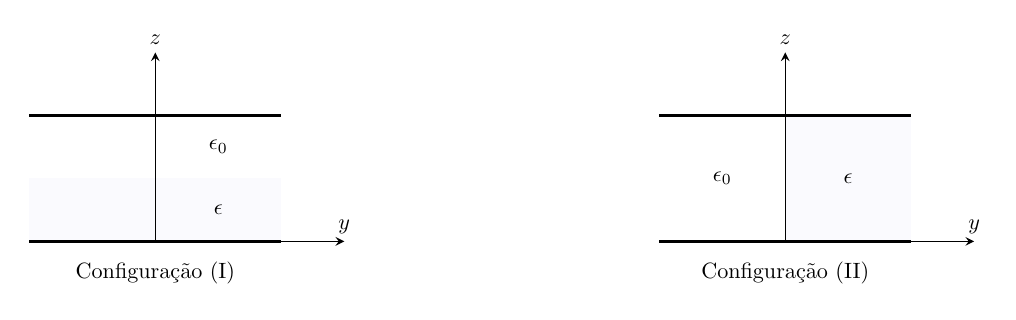
\begin{tikzpicture}[scale=0.8, every node/.style={scale=0.8}]
            \fill[Lavender!20] (0,0) rectangle (4,1);
            \draw[very thick] (0,2) -- (4,2);
            \draw[very thick] (0,0) -- (4,0);

            \node at (3,1.5) {$\epsilon_0$};
            \node at (3,0.5) {$\epsilon$};

            \draw[-stealth] (2,0) -- (2,3) node[above] {$z$};
            \draw[-stealth] (0,0) -- (5,0) node[above] {$y$};

            \node at (2,-0.5) {Configuração (I)};
            \begin{scope}[xshift=10cm]
                \fill[Lavender!20] (2,0) rectangle (4,2);
                \draw[very thick] (0,2) -- (4,2);
                \draw[very thick] (0,0) -- (4,0);

                \node at (1,1) {$\epsilon_0$};
                \node at (3,1) {$\epsilon$};

                \draw[-stealth] (2,0) -- (2,3) node[above] {$z$};
                \draw[-stealth] (0,0) -- (5,0) node[above] {$y$};

                \node at (2,-0.5) {Configuração (II)};
            \end{scope}
        \end{tikzpicture}
    \end{center}

    Calcule a energia eletrostática armazenada em toda a região entre as placas em cada configuração. Dado que \(k > 1\), em qual das duas configurações a energia é maior?
\end{exercício}
\begin{proof}[Resolução para a configuração (I)]
    Como o potencial satisfaz a equação de Laplace no interior das placas e é invariante por translações em \(x\) e em \(y\), segue que
    \begin{equation*}
        \phi(\vetor{\x})=\begin{cases}
            B\inner{\vetor{e}_z}{\vetor{\x}} + (A-B)\frac{d}{2},&\text{se }\inner{\vetor{e}_z}{\vetor{\x}} \in (\frac{d}{2}, d]\\
            A\inner{\vetor{e}_z}{\vetor{\x}},&\text{se }\inner{\vetor{e}_z}{\vetor{\x}} \in [0,\frac{d}{2}]
        \end{cases},
    \end{equation*}
    onde já utilizamos a continuidade do potencial em \(z = 0\) e \(z = \frac{d}{2}\). Como \(\phi(d) = \phi_0\), temos
    \begin{equation*}
        Bd + Ad= 2\phi_0,
    \end{equation*}
    e como não há cargas livres na interface com o dielétrico, temos
    \begin{equation*}
        -\epsilon_0 \diffp{\phi}{z}[z=\frac{d}{2}^+] + \epsilon \diffp{\phi}{z}[z=\frac{d}{2}^-] = 0 \implies -\epsilon_0 B + \epsilon A = 0.
    \end{equation*}
    Resolvendo o sistema de equações lineares, encontramos
    \begin{equation*}
        A = \frac{2\epsilon_0 \phi_0}{d \epsilon + d \epsilon_0} = \frac{2 \phi_0}{(k + 1)d} \quad\text{e}\quad B = k A = \frac{2 k \phi_0}{(k + 1)d},
    \end{equation*}
    portanto
    \begin{equation*}
        \phi(\vetor{\x}) = \begin{cases}
            \frac{2\phi_0}{(k+1)d}\inner{\vetor{e}_z}{\vetor{\x}},&\text{se }\inner{\vetor{e}_z}{\vetor{\x}} \in [0,\frac{d}{2}]\\
            \frac{2k \phi_0}{(k+1)d}\inner{\vetor{e}_z}{\vetor{\x}} + \frac{1-k}{k+1}\phi_0, &\text{se }\inner{\vetor{e}_z}{\vetor{\x}} \in (\frac{d}{2},d]
        \end{cases}
    \end{equation*}
    é o potencial entre as placas. Portanto, o campo elétrico é dado por
    \begin{equation*}
        \vetor{E}(\vetor{\x}) = \begin{cases}
            -\frac{2\phi_0}{(k+1)d}\vetor{e}_z,&\text{se }\inner{\vetor{e}_z}{\vetor{\x}}\in [0,\frac{d}{2}]\\
            -\frac{2k\phi_0}{(k+1)d}\vetor{e}_z,&\text{se }\inner{\vetor{e}_z}{\vetor{\x}}\in (\frac{d}{2},d]
        \end{cases},
    \end{equation*}
    donde segue que
    \begin{equation*}
        \vetor{D}(\vetor{\x}) = -\frac{2 \epsilon \phi_0}{(k + 1)d}\vetor{e}_z,\quad\text{se }\inner{\vetor{e}_z}{\vetor{\x}} \in [0, d].
    \end{equation*}
    Dessa forma, a densidade de energia na região entre as placas é
    \begin{equation*}
        u_\mathrm{E} = \frac12 \inner{\vetor{D}}{\vetor{E}} = \begin{cases}
            \frac{2\epsilon \phi_0^2}{(k+1)^2d^2},&\text{se }\inner{\vetor{e}_z}{\vetor{\x}}\in [0,\frac{d}{2}]\\
            \frac{2k \epsilon \phi_0^2}{(k+1)^2d^2},&\text{se }\inner{\vetor{e}_z}{\vetor{\x}}\in (\frac{d}{2},d]
        \end{cases}
    \end{equation*}
    e
    \begin{equation*}
        U_\mathrm{E}^{\mathrm{(I)}} = \frac{L^2 \epsilon \phi_0^2}{(k+1)d}
    \end{equation*}
    é a energia eletrostática armazenada na região entre as placas.
\end{proof}

\begin{proof}[Resolução para a configuração (II)]
    Como o potencial satisfaz a equação de Laplace nas regiões com e sem dielétrico, temos
    \begin{equation*}
        \phi(\vetor{\x}) = \frac{\phi_0}{d}\inner{\vetor{e}_z}{\vetor{\x}},\quad\text{se }\inner{\vetor{e}_z}{\vetor{\x}} \in [0,d],
    \end{equation*}
    portanto o campo elétrico é
    \begin{equation*}
        \vetor{E}(\vetor{\x}) = -\frac{\phi_0}{d}\vetor{e}_z,\quad\text{se }\inner{\vetor{e}_z}{\vetor{\x}} \in [0,d],
    \end{equation*}
    e segue que
    \begin{equation*}
        \vetor{D}(\vetor{\x}) = \begin{cases}
            - \frac{\epsilon_0\phi_0}{d}\vetor{e}_z,&\text{se }\inner{\vetor{e}_y}{\vetor{\x}} < 0\text{ e }\inner{\vetor{e}_z}{\vetor{\x}} \in [0,d]\\
            - \frac{k\epsilon_0\phi_0}{d}\vetor{e}_z,&\text{se }\inner{\vetor{e}_y}{\vetor{\x}} > 0\text{ e }\inner{\vetor{e}_z}{\vetor{\x}} \in [0,d]
        \end{cases}.
    \end{equation*}
    Dessa forma, a densidade de energia na região entre as placas é
    \begin{equation*}
        u_\mathrm{E} = \frac12\inner{\vetor{D}}{\vetor{E}} = \begin{cases}
            \frac{\epsilon_0\phi_0^2}{2d^2},&\text{se }\inner{\vetor{e}_y}{\vetor{\x}} < 0\text{ e }\inner{\vetor{e}_z}{\vetor{\x}} \in [0,d]\\
            \frac{k\epsilon_0\phi_0^2}{2d^2},&\text{se }\inner{\vetor{e}_y}{\vetor{\x}} > 0\text{ e }\inner{\vetor{e}_z}{\vetor{\x}} \in [0,d]
        \end{cases}
    \end{equation*}
    e
    \begin{equation*}
        U_\mathrm{E}^{\mathrm{(II)}} = \frac{L^2 (k+1)\epsilon_0 \phi_0^2}{4d}
    \end{equation*}
    é a energia eletrostática armazenada na região entre as placas. Notemos que para \(k > 1\) temos
    \begin{equation*}
        \frac{U_\mathrm{E}^{\mathrm{(II)}}}{U_\mathrm{E}^{\mathrm{(I)}}} = \frac{(k+1)^2}{4k} > 1,
    \end{equation*}
    portanto a energia armazenada na configuração (II) é maior do que na configuração (I).
\end{proof}
